\documentclass[main.tex]{subfiles}
\begin{document}

\chapter{Experimentation}

In order to test the proposed framework, an implementation is provided. The framework implementation is targeted at the Digilent Nexys 4 FPGA development board, displayed in figure \ref{fig:nexys4}. This board contains a Xilinx Artix-7 series FPGA and is equipped with various I/O devices. The development board is connected with the PC through USB. This USB connection is used in order to setup a serial communication channel between the PC and the FPGA.

\begin{figure}
\centering
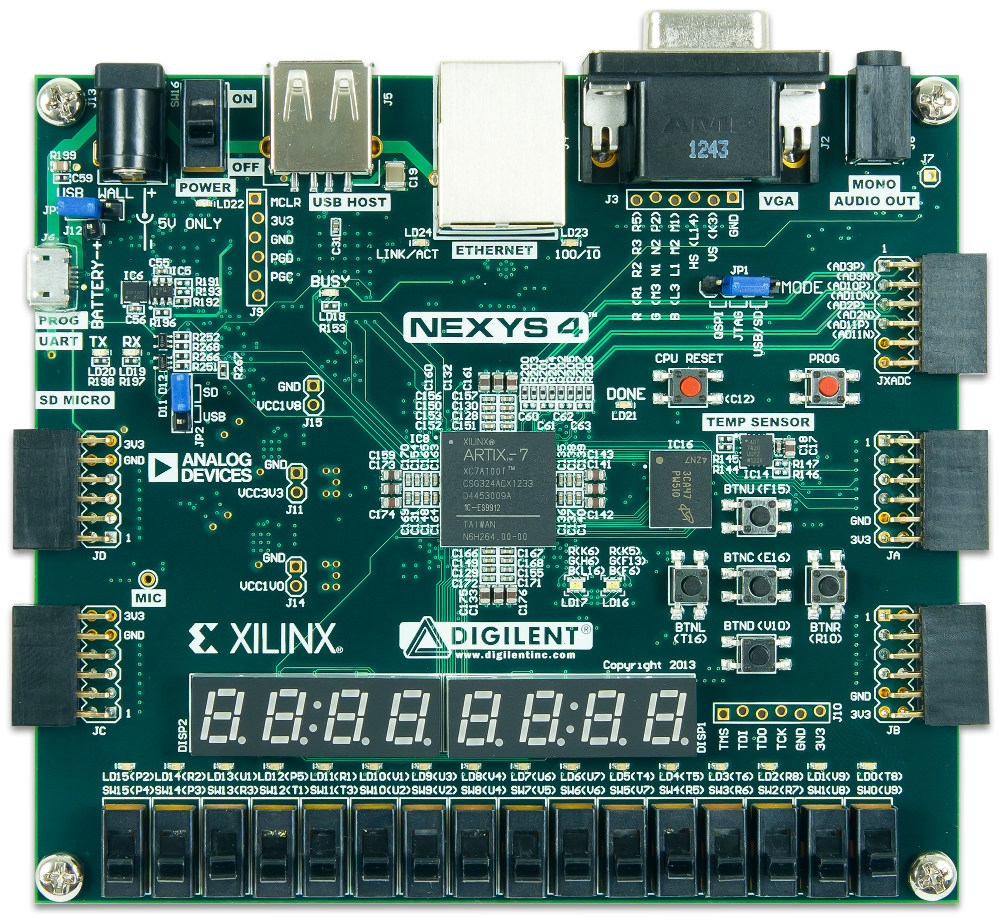
\includegraphics[width=0.7\textwidth]{img/nexys4-small}
\caption{Digilent Nexys 4 Artix-7 FPGA development board}
\label{fig:nexys4}
\end{figure}


\chapter{Results}
\begin{itemize}
    \item validate through proof of concept, multiple examples of use cases
    \item Comparison to other methods
    \item Analyse behaviour of wrapper in terms of size and performance
    \item Analyse the appropriateness of an address space as a unit of abtraction and interaction
    \item Validate the appropriateness of design decisions in the model, such as the adoption of address space
    
\end{itemize}

\end{document}